\documentclass{beamer}

\usepackage[francais]{babel}
\usepackage{amsmath}
\usepackage{amssymb}
\usepackage[T1]{fontenc}
\usepackage[utf8]{inputenc}
\usepackage{latexsym}
\usepackage{stmaryrd}
\usepackage{graphicx}
\usepackage{amsfonts}

\linespread{1.7}

\title{Réforme du quotient conjugual}

\begin{document}

\begin{frame}
\titlepage
\end{frame}

\begin{frame}
\frametitle{Plan}
\tableofcontents
\end{frame}

\section{Motivations de l'étude}

\begin{frame}
\frametitle{Motivations de l'étude}
\begin{itemize}
\item Contexte : réforme de l'impôt sur le revenu annoncée

\item Système actuel : 

\begin{itemize}

\item IR conjugalisé pour couples mariés ou pacsés 

\begin{itemize}

\item Système de quotient conjugal avec deux parts

\end{itemize}

\item Imposition séparée au titre de l'IR pour concubins

\item CSG individualisée

\end{itemize}

\end{itemize}
\end{frame}

\begin{frame}
\frametitle{Motivations de l'étude}
\framesubtitle{Fonctionnement du quotient conjugal}

\begin{itemize}

\item Impôt = BarêmeIR($\dfrac{\text{Revenu fiscal}}{2}$) $\times$ 2.

\begin{itemize}

\item $\to$ taux d'imposition d'un couple de revenu R = taux d'imposition d'un célibataire de revenu $\dfrac{R}{2}$

\item $\to$ IR total payé par un couple de revenu R $\leq$ l'IR payé par deux célibataires de revenu $\dfrac{R}{2}$

\item $\to$ Gain à l'imposition commune : fonction croissante de la différence de revenus entre les deux membres du couple

\begin{itemize}

\item Due à l'imposition à la moyenne et à la progressivité de l'IR

\end{itemize}

\end{itemize}

\end{itemize}

\end{frame}

\begin{frame}

\frametitle{Motivations de l'étude}

\framesubtitle{Problèmes liés au système de quotient conjugal}

\begin{itemize}

\item Le QC donne un avantage trop important aux couples par rapport aux célibataires.

\begin{itemize}
\item Parts fiscales = 2 pour un couple
\item Unités de consommation = 1,5 $<$ 2 (économies d'échelles)
\end{itemize}

\item Le QC favorise la monoactivité (problème : pas de droits sociaux propres pour le conjoint aux revenus les plus faibles)

\item Le QC ne prend pas en compte l'apport de la production domestique en termes de niveau de vie

\end{itemize}

\end{frame}

\begin{frame}

\frametitle{Motivations de l'étude}

\framesubtitle{Proposition de réforme}

\begin{itemize}

\item Le QC est donc trop généreux, ce qui nous amène à proposer une réforme

\item Réforme :

\begin{enumerate}

\item Faire passer la part du conjoint de 1 à 0,5

\item Laisser le choix à chaque couple (marié ou non) entre déclaration commune et déclarations séparées

\end{enumerate}

\end{itemize}

\end{frame}

\section{Présentation des résultats}

\begin{frame}
\frametitle{Présentation des résultats}
\framesubtitle{Gain à l'imposition commune dans la législation actuelle}
\includegraphics[width=8cm]{GainImpComm1.png}
\end{frame}

\begin{frame}
\frametitle{Présentation des résultats}
\framesubtitle{Gain à l'imposition commune sous nouveau barême de QC}
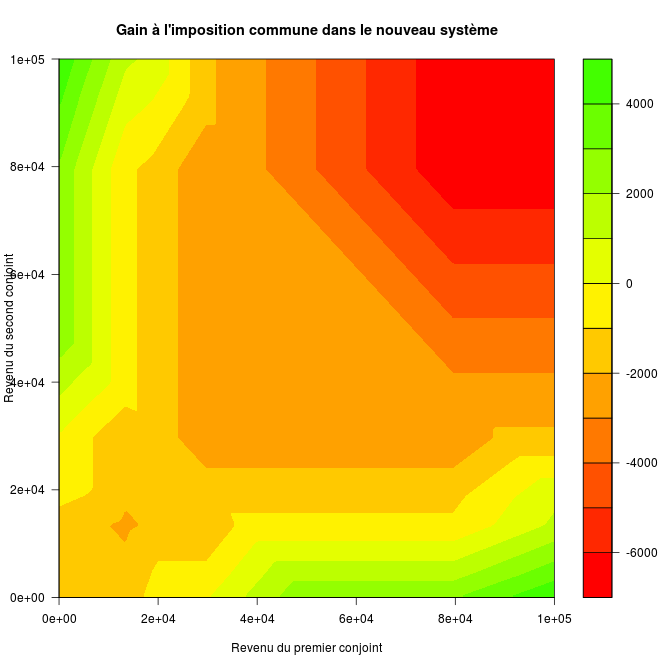
\includegraphics[width=8cm]{GainImpComm2.png}
\end{frame}

\begin{frame}
\frametitle{Présentation des résultats}
\framesubtitle{Différence d'IRPP entre législation actuelle et nouveau barême pour les couples mariés}
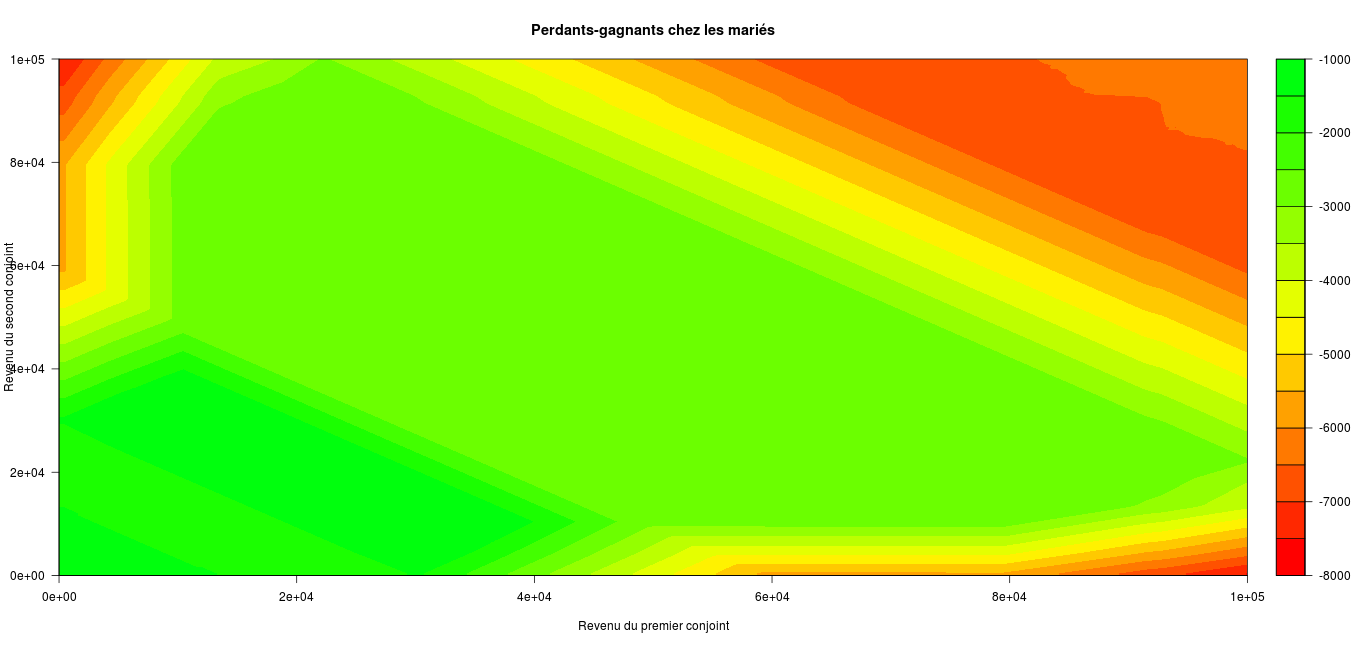
\includegraphics[width=11cm]{perdantsmar.png}
\end{frame}

\begin{frame}
\frametitle{Présentation des résultats}
\framesubtitle{Différence d'IRPP entre législation actuelle et nouveau barême pour les concubins}
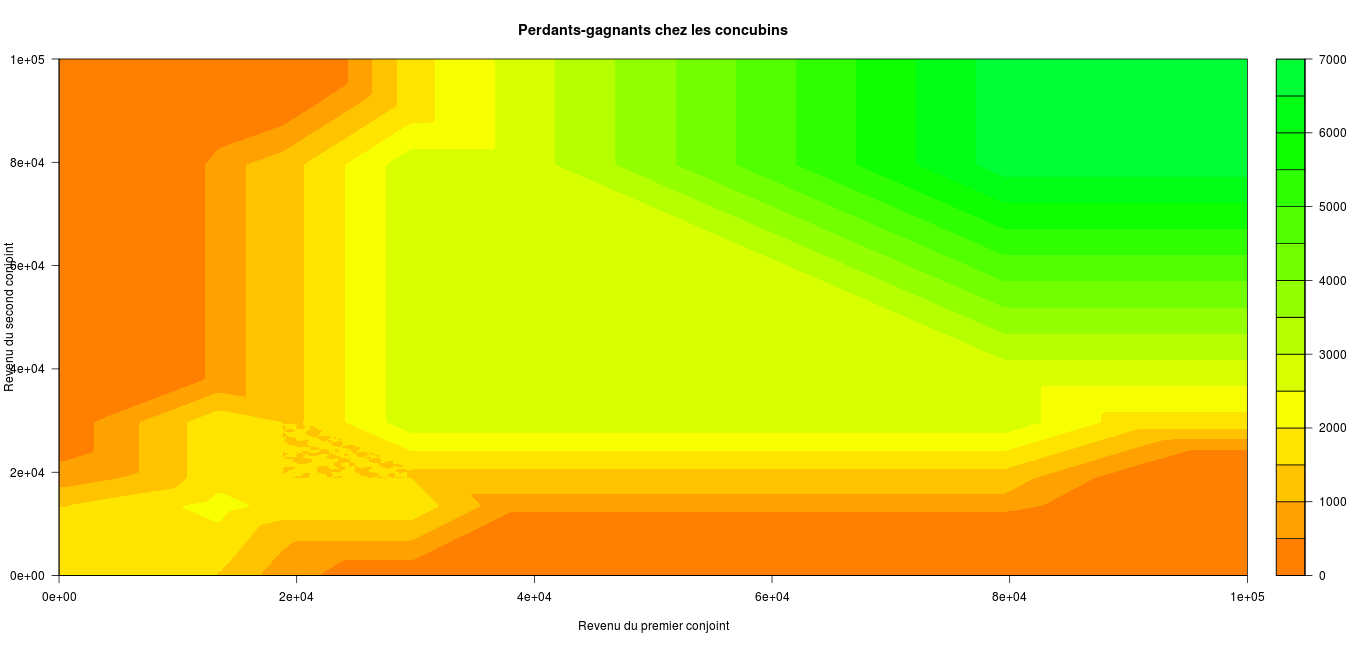
\includegraphics[width=11cm]{perdantsconc.png}
\end{frame}

\section{Pistes de recherches ultérieures}

\begin{frame}
\frametitle{Pistes de recherches ultérieures}

\begin{itemize}
\item Modèle actuel : couple marié sans enfants. Etendre la comparaison aux couples avec enfants. 

\begin{itemize}
\item Problème : à qui attribuer l'enfant ?
\end{itemize}


\end{itemize}

\end{frame}

\end{document}
